% Created: 2020-01-10, John Miller

%==========================================================
%=========== Document Setup  ==============================

% Formatting defined by class file
\documentclass[11pt]{article}

% ---- Document formatting ----
\usepackage[margin=1in]{geometry}	% Narrower margins
\usepackage{booktabs}				% Nice formatting of tables
\usepackage{graphicx}				% Ability to include graphics

%\setlength\parindent{0pt}	% Do not indent first line of paragraphs 
\usepackage[parfill]{parskip}		% Line space b/w paragraphs
%	parfill option prevents last line of pgrph from being fully justified

% Parskip package adds too much space around titles, fix with this
\RequirePackage{titlesec}
\titlespacing\section{0pt}{8pt plus 4pt minus 2pt}{3pt plus 2pt minus 2pt}
\titlespacing\subsection{0pt}{4pt plus 4pt minus 2pt}{-2pt plus 2pt minus 2pt}
\titlespacing\subsubsection{0pt}{2pt plus 4pt minus 2pt}{-6pt plus 2pt minus 2pt}

% ---- Hyperlinks ----
\usepackage[colorlinks=true,urlcolor=blue]{hyperref}	% For URL's. Automatically links internal references.

% ---- Code listings ----
\usepackage{listings} 					% Nice code layout and inclusion
\usepackage[usenames,dvipsnames]{xcolor}	% Colors (needs to be defined before using colors)

% Define custom colors for listings
\definecolor{listinggray}{gray}{0.98}		% Listings background color
\definecolor{rulegray}{gray}{0.7}			% Listings rule/frame color

% Style for Verilog
\lstdefinestyle{Verilog}{
	language=Verilog,					% Verilog
	backgroundcolor=\color{listinggray},	% light gray background
	rulecolor=\color{blue}, 			% blue frame lines
	frame=tb,							% lines above & below
	linewidth=\columnwidth, 			% set line width
	basicstyle=\small\ttfamily,	% basic font style that is used for the code	
	breaklines=true, 					% allow breaking across columns/pages
	tabsize=3,							% set tab size
	commentstyle=\color{gray},	% comments in italic 
	stringstyle=\upshape,				% strings are printed in normal font
	showspaces=false,					% don't underscore spaces
}

% How to use: \Verilog[listing_options]{file}
\newcommand{\Verilog}[2][]{%
	\lstinputlisting[style=Verilog,#1]{#2}
}




%======================================================
%=========== Body  ====================================
\begin{document}

\title{ELC 2137 Lab 5: Intro to Verilog}
\author{Trevor Jackson, Carlos Hernandez, and Makenna Meyers}

\maketitle


\section*{Summary}

This lab was an introduction to coding with Verilog. We learned to code the half adder, full adder, and adder/subtractor circuits that we had assembled with wires in previous labs. The codes for the adders and their test benches can be found below in Codes \ref{code:half adder}, \ref{code:half adder test bench}, \ref{code:full adder}, \ref{code:full adder test bench}, \ref{code:adder/subtractor}, and \ref{code:adder/subtractor test bench}. Expected Results Tables (ERTs) and simulation waveforms for each adder can be found in Figures \ref{fig:sim_with_table_HA}, \ref{fig:sim_with_table_FA}, and \ref{fig:sim_with_table_SUB}. In addition to writing and testing the code for the adders, block diagrams were drawn to illustrate the inputs, outputs, wires, and gates involved with each circuit. Those can be found in Figures \ref{fig:half_adder_diagram}, \ref{fig:full_adder_diagram}, and \ref{fig:subtractor_diagram}.

\section*{Q\&A}

\begin{enumerate}
	\item What is one thing you still don't understand about Verilog?
	
	What is the most efficient way to implement the logic gates?
	
\end{enumerate}

\section*{Results}
\begin{figure}\centering
	\begin{tabular}{l|c||c|c}
		A & B & C & S \\
		\midrule
		0 & 0 & 0 & 0 \\
		0 & 1 & 0 & 1 \\
		1 & 0 & 0 & 1 \\
		1 & 1 & 1 & 0 \\
		\bottomrule
	\end{tabular} 
	
	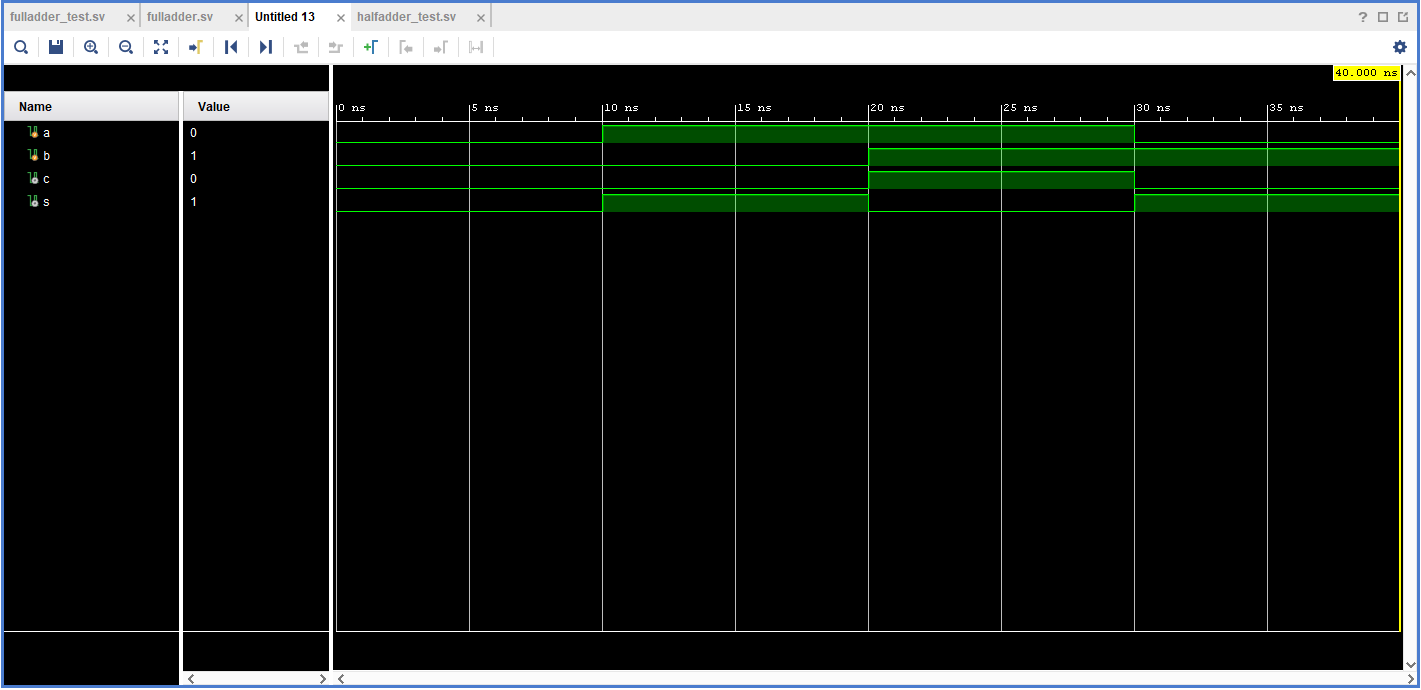
\includegraphics[width=0.8\textwidth,trim=0cm 12cm 0.3cm 1.5cm,clip]{half_adder_simwave}
	\caption{Half Adder ERT and Simulation Waveform}
	\label{fig:sim_with_table_HA}
\end{figure}

\begin{figure}\centering
	\begin{tabular}{l|c|c||c|c}
		Cin & A & B & Cout & S \\
		\midrule
		0 & 0 & 0 & 0 & 0 \\
		0 & 0 & 1 & 0 & 1 \\
		0 & 1 & 0 & 0 & 1 \\
		0 & 1 & 1 & 1 & 0 \\
		1 & 0 & 0 & 0 & 1 \\
		1 & 0 & 1 & 1 & 0 \\
		1 & 1 & 0 & 1 & 0 \\
		1 & 1 & 1 & 1 & 1 \\
		\bottomrule
	\end{tabular} 
	
	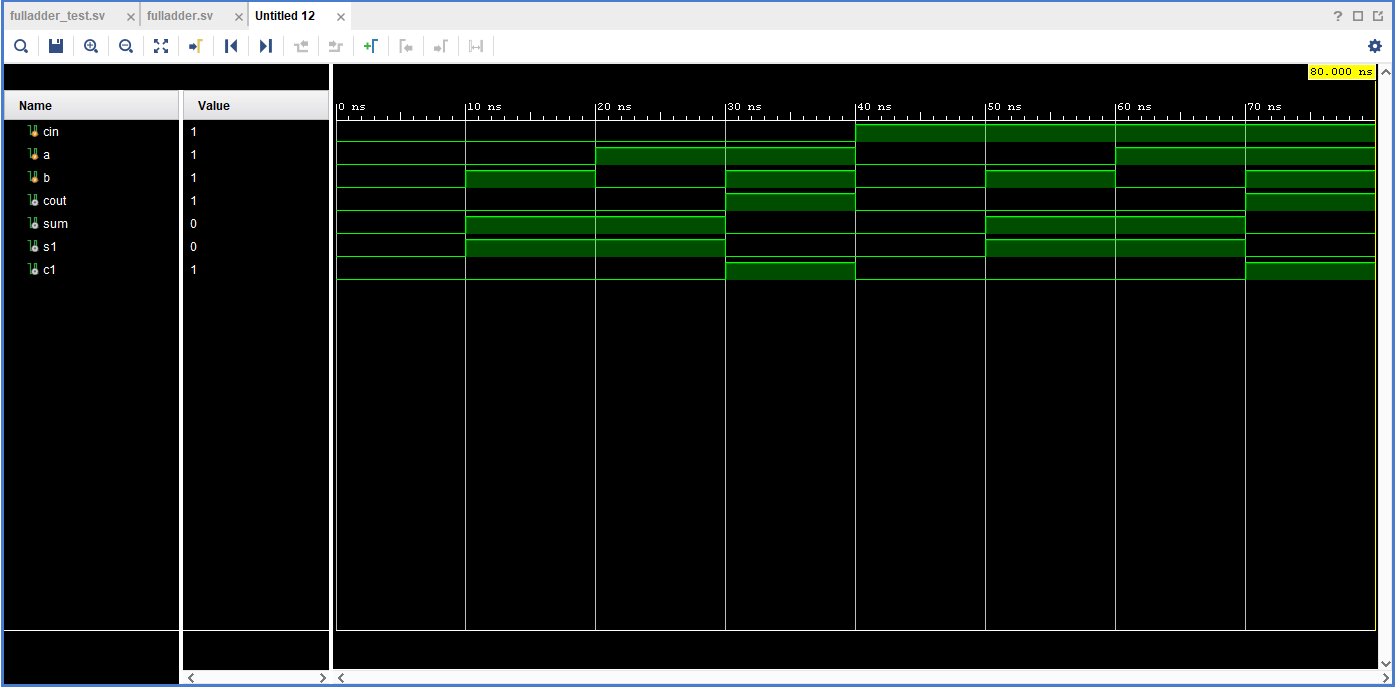
\includegraphics[width=0.8\textwidth,trim=0cm 10cm 0.3cm 1.5cm,clip]{full_adder_simwave}
	\caption{Full Adder ERT and Simulation Waveform}
	\label{fig:sim_with_table_FA}
\end{figure}

\begin{figure}\centering
	\begin{tabular}{l|c||c|c|c}
		A & B & Cout & S2 & S1 \\
		\midrule
		00 & 01 & 1 & 1 & 1 \\
		00 & 10 & 1 & 1 & 0 \\
		00 & 11 & 1 & 0 & 1 \\
		01 & 01 & 0 & 0 & 0 \\
		10 & 01 & 0 & 0 & 1 \\
		10 & 00 & 0 & 1 & 0 \\
		\bottomrule
	\end{tabular} 
	
	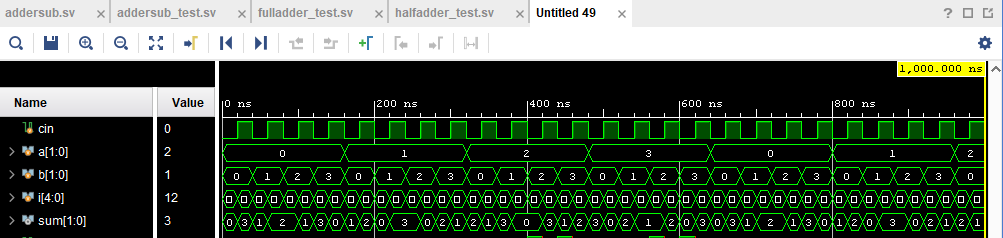
\includegraphics[width=0.8\textwidth,trim=0cm 0cm 0.3cm 1.5cm,clip]{addersub_simwave1}
	\caption{Adder/Subtractor ERT and Simulation Waveform}
	\label{fig:sim_with_table_SUB}
\end{figure}

\begin{figure}\centering
	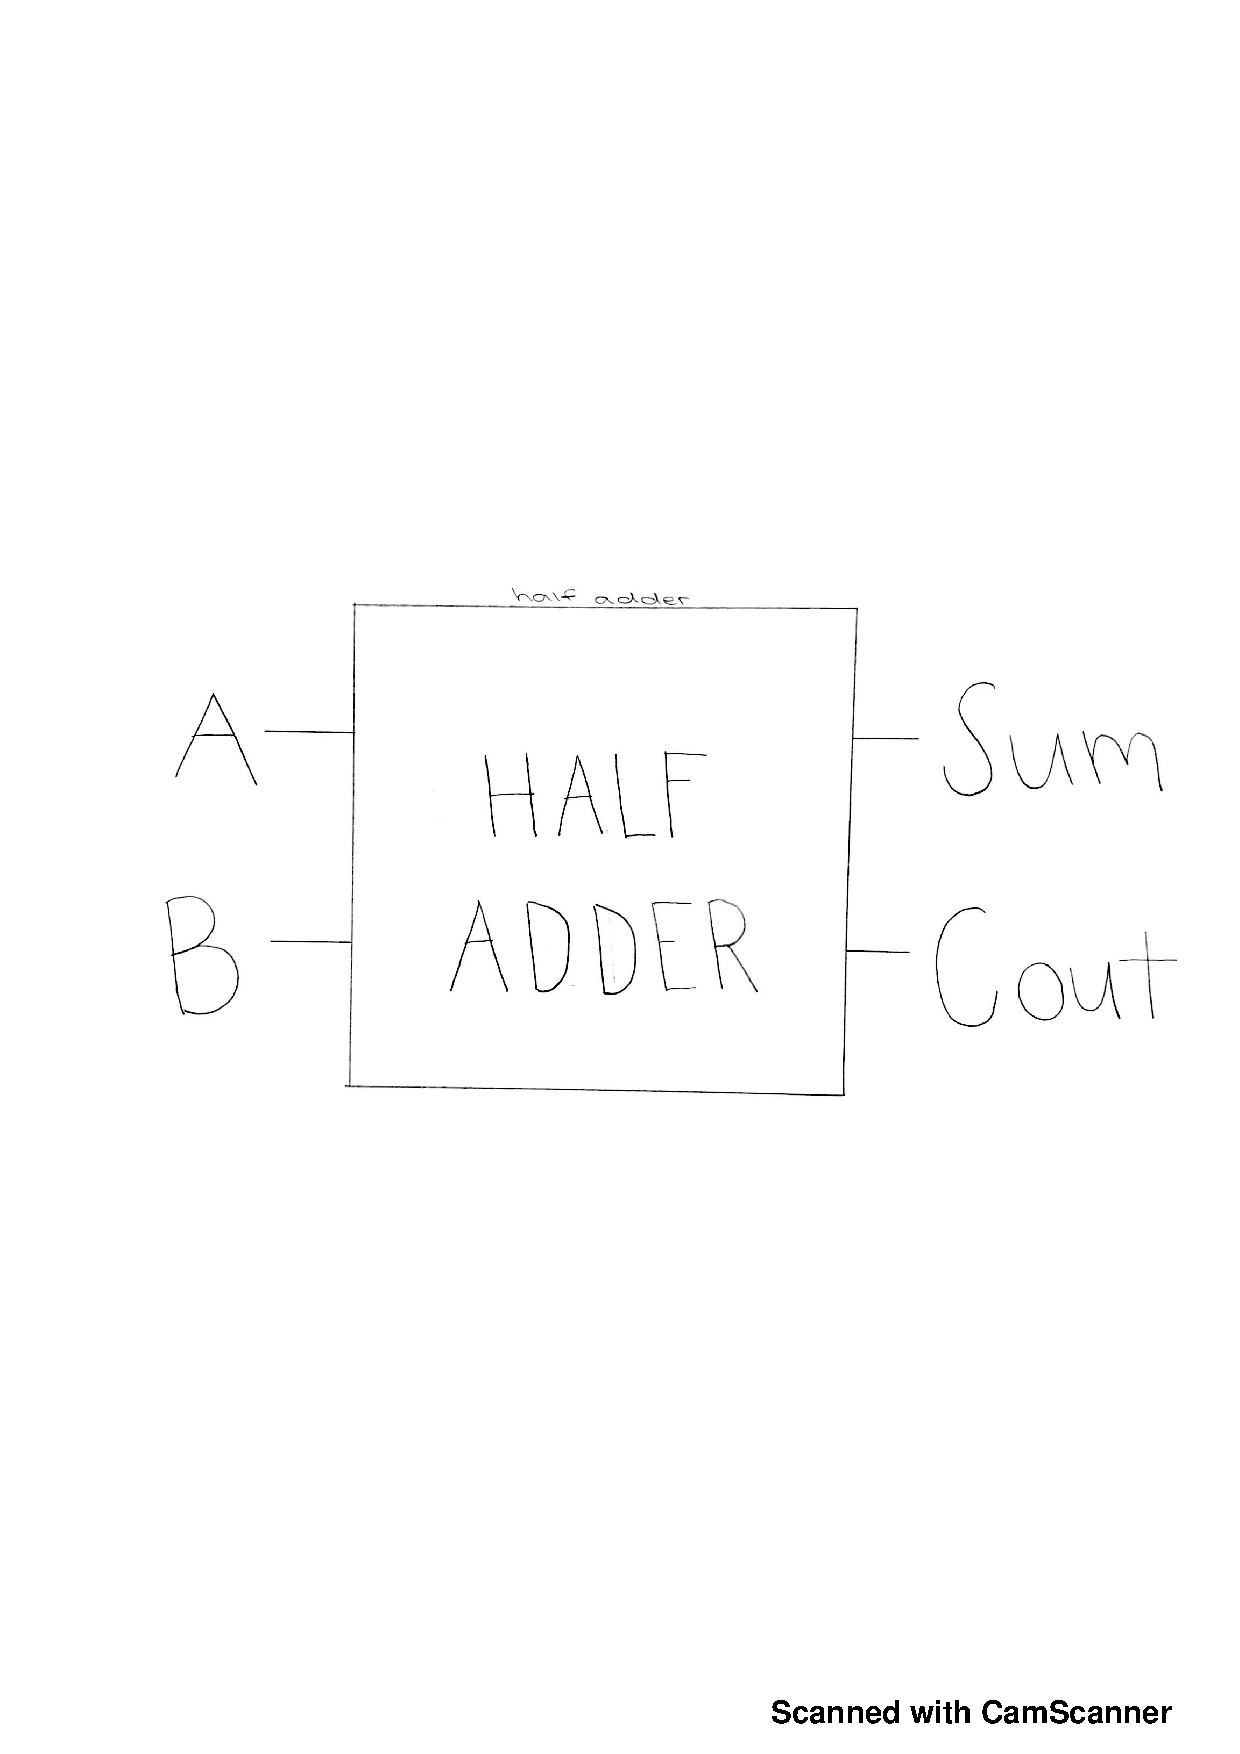
\includegraphics[width=0.8\textwidth,trim=0cm 11cm 0cm 9.5cm,clip]{half_adder_block_diagram}
	\caption{Half Adder Block Diagram}
	\label{fig:half_adder_diagram}	
\end{figure}

\begin{figure}\centering
	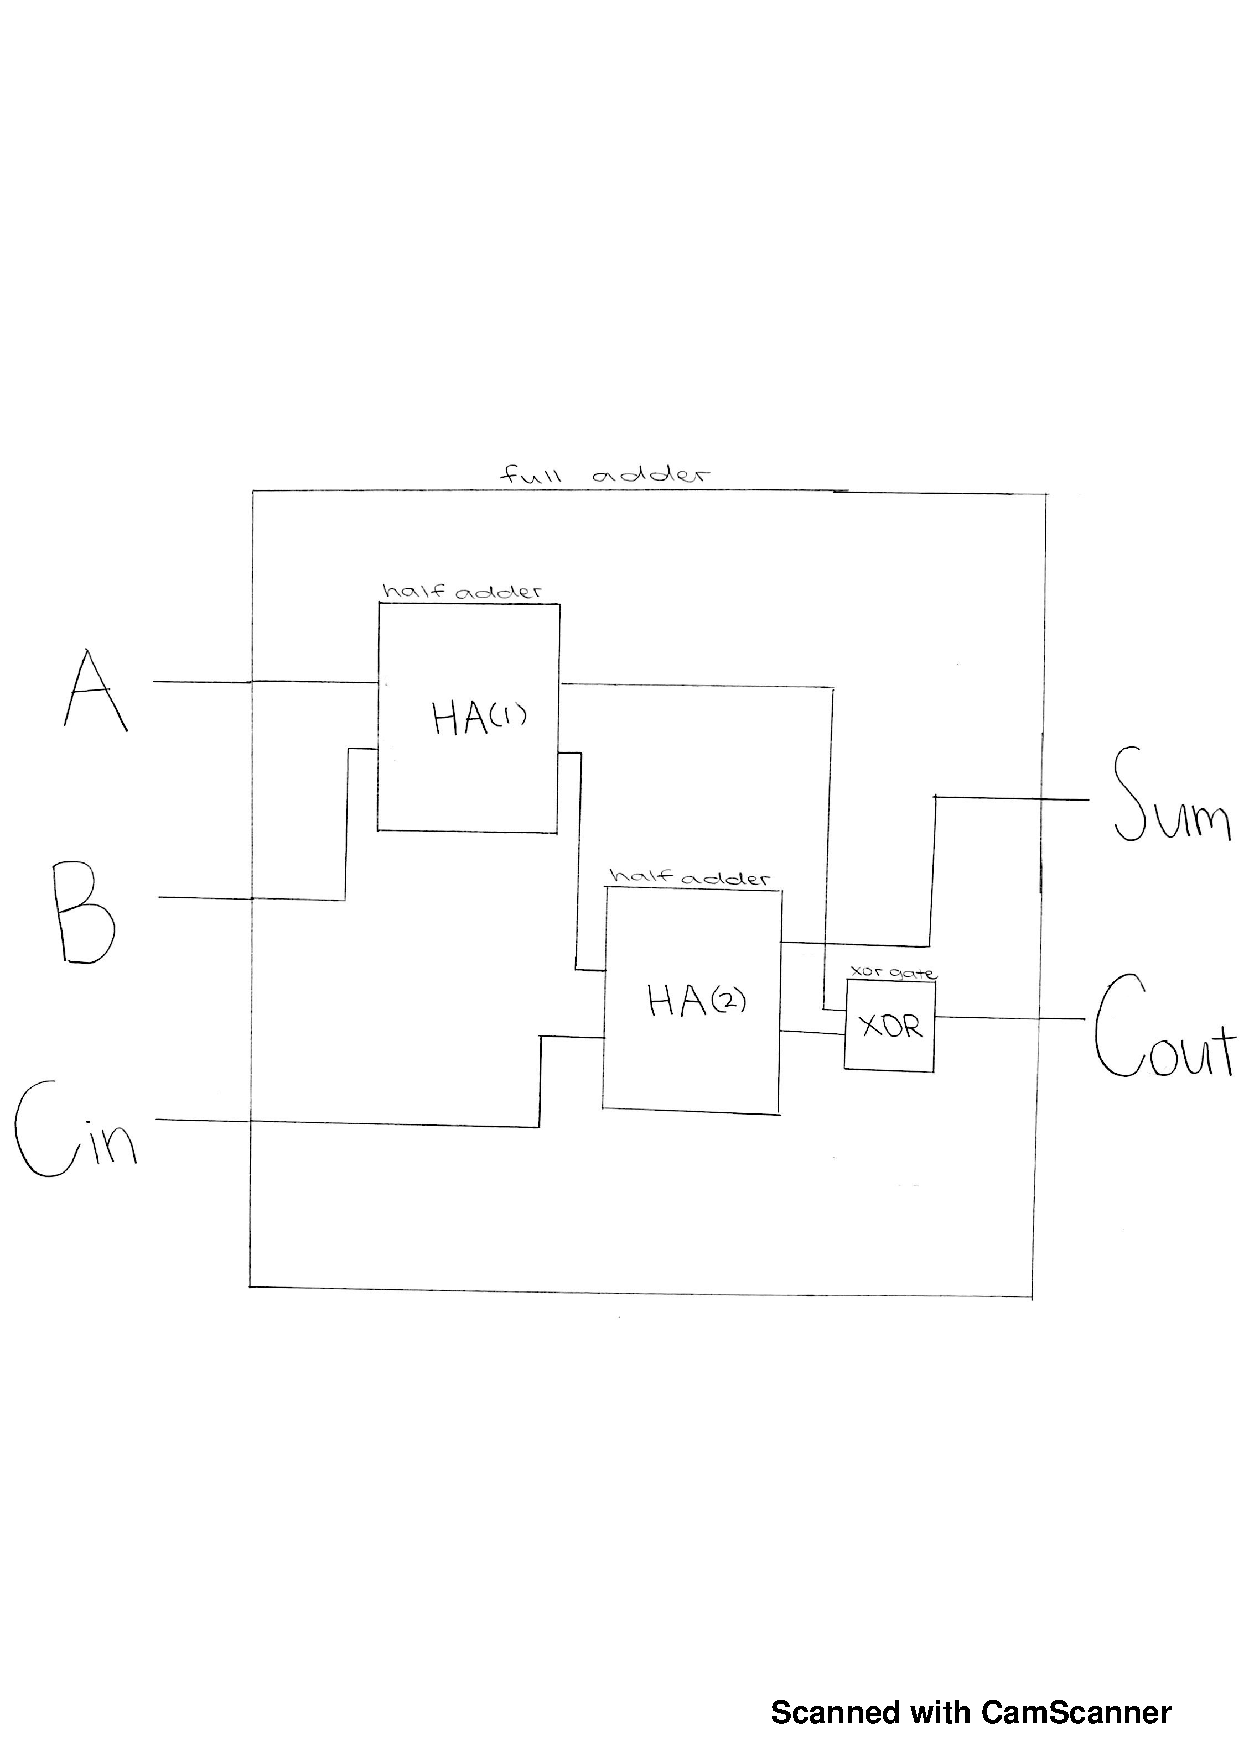
\includegraphics[width=0.8\textwidth,trim=0cm 7.5cm 0cm 7.5cm,clip]{full_adder_block_diagram}
	\caption{Full Adder Block Diagram}
	\label{fig:full_adder_diagram}	
\end{figure}

\begin{figure}\centering
	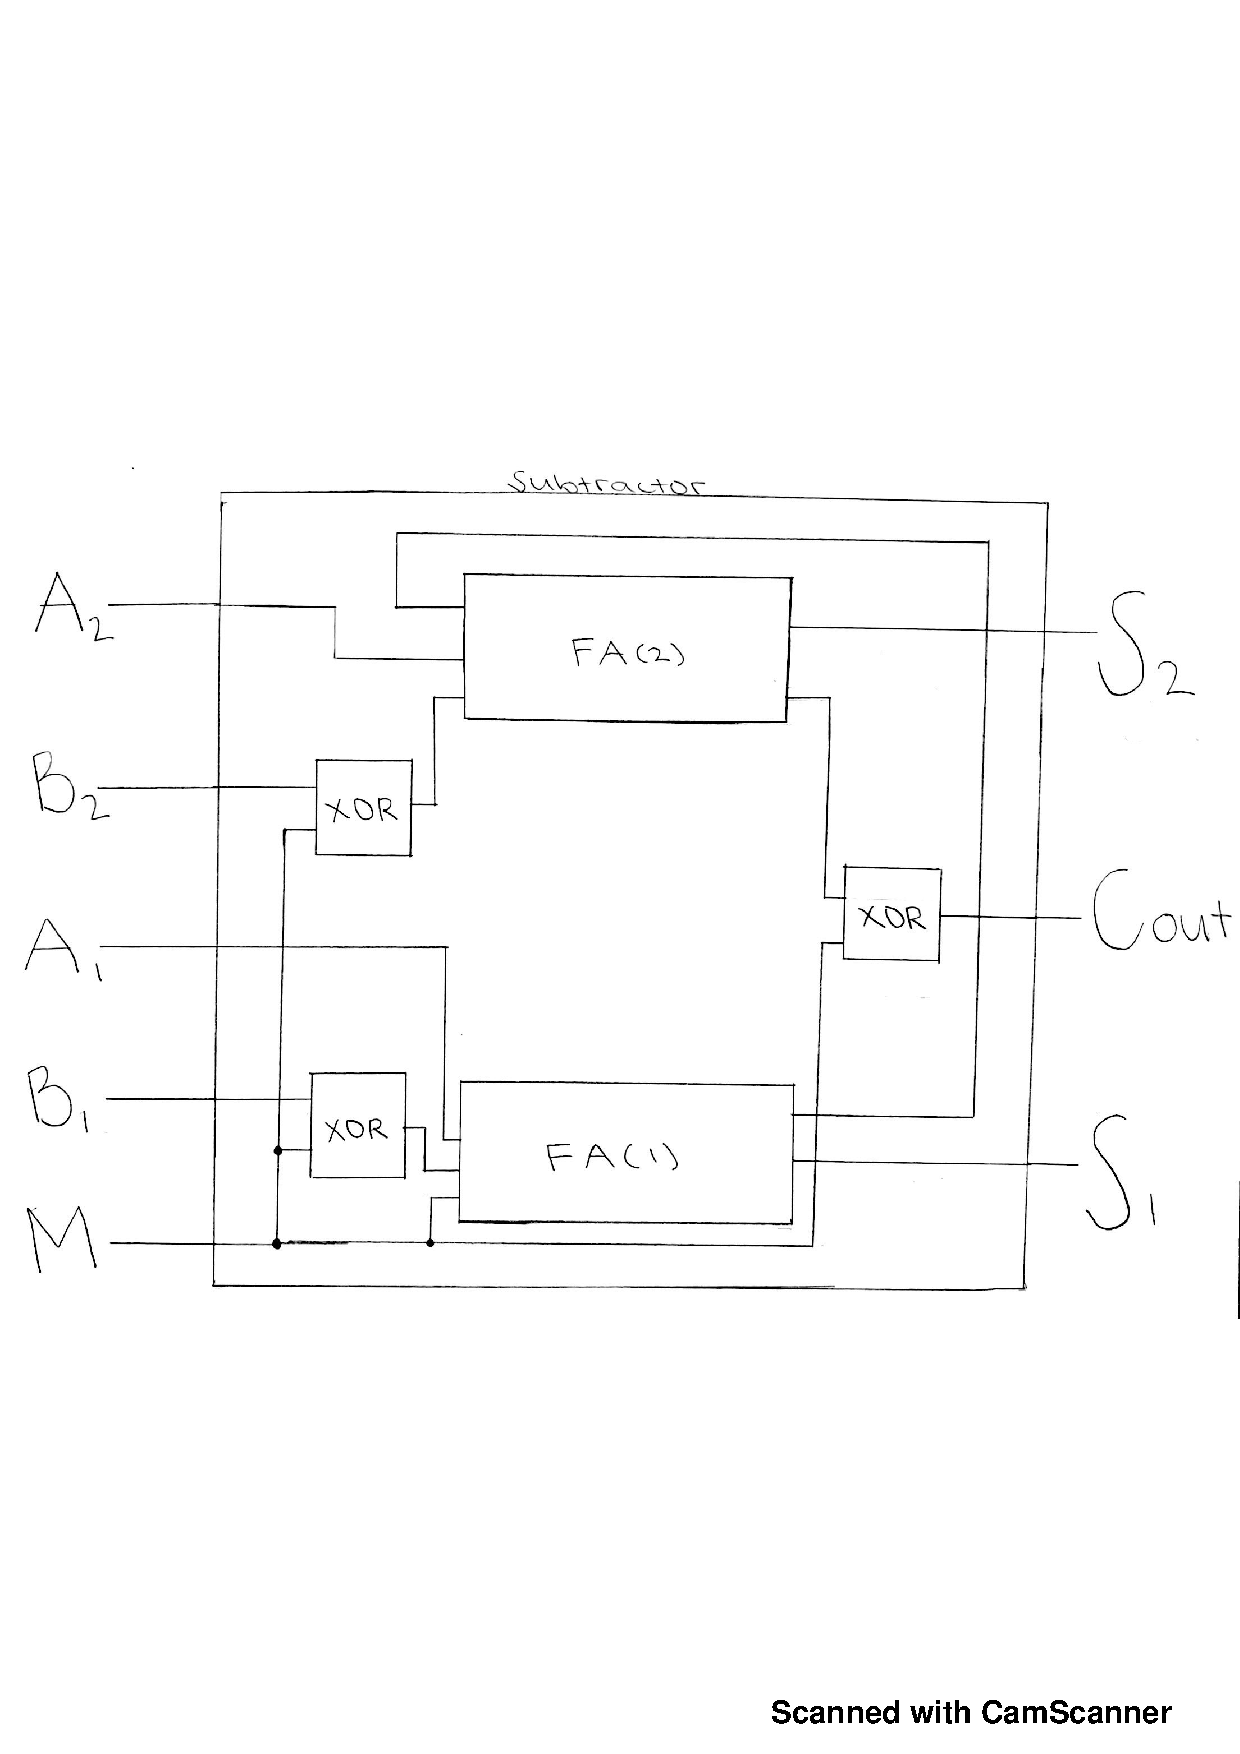
\includegraphics[width=0.8\textwidth,trim=0cm 7.5cm 0cm 7.5cm,clip]{subtractor_block_diagram} 
	\caption{Adder/Subtractor Block Diagram}
	\label{fig:subtractor_diagram}
\end{figure}

\clearpage

\section*{Code}

\Verilog[caption=Half Adder Code,label=code:half adder]{halfadder.sv}

\Verilog[caption=Half Adder Test Bench Code,label=code:half adder test bench]{halfadder_test.sv}

\Verilog[caption=Full Adder Code,label=code:full adder]{fulladder.sv}

\Verilog[caption=Full Adder Test Bench Code,label=code:full adder test bench]{fulladder_test.sv}

\Verilog[caption=Adder/Subtractor Code,label=code:adder/subtractor]{addersub2.sv}

\Verilog[caption=Adder/Subtractor Test Bench Code,label=code:adder/subtractor test bench]{addersub_test2.sv}

\end{document}
